\chapter{Amplifier modelling}

\section{Pre-distortion}

\begin{figure}[H]
\centering 
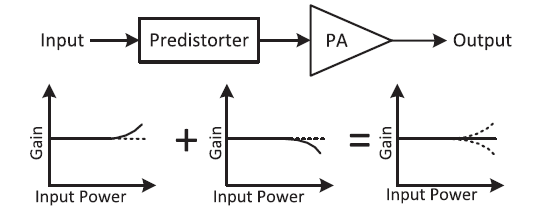
\includegraphics[scale = 0.7]{figures/ch1/predistortion_consept.png}
\caption{Consept of predistortion \citep{guo2015}}
\label{fig:pre_cons}
\end{figure}

In figure \ref{fig:pre_cons} the consept of Digital Pre-Distortion (DPD) is depicted. DPD is a way to "distort" the incomming signal with the inverse transfer-function of the amplifier. For example the gain of the amplifier is ideally linear in the small-signal region and gets non-linear at higher signal levels. To overcome this, a block called the predistorter inverses this non-linear curve which is the exact inverse of the PA, then a linear amplification can be achieved at the final PA output. But to archive this inverse of the PA all the non-linear effects has to be accounted for including memory effects. 

\section{DPD models}


\subsubsection{Weiner}
A simpel model to include memory effects is the Weiner model, which consists of a linear filter $h(m)$ followed by $a_k$ which is the polynomial coefficients of the non-linearity. The model is given by equation \ref{eq:wiener}

\begin{equation}\label{eq:wiener}
y_{wiener}(n) = \sum_{k=1}^{K} a_k [\sum_{m=0}^{M-1}h(m)x(n-m)]^k
\end{equation} 

It is seen that the output consists of the sum of the non-linear response multiplied with the sum of the input with the former input multiplied with a filter. The Weiner model is one of the simplest ways to combine memory effects with non-linearity but unfortunately it does not provide good results for modelling a power amplifier. 

 
\subsubsection{Hammerstein} 
Another simple model is the Hammerstein model which is given by equation \ref{eq:hammer}

\begin{equation} \label{eq:hammer}
y_{hammerstein}(n) = \sum_{m=0}^{M-1}g(m)\sum_{k=1}^{K}a_k x^k(n-m)
\end{equation} 

Which is formed by a non-linearity followed by a linear filter. It is seen that the output consist of the sum of the linear filter $g(m)$ multiplied with the sum of the filter coefficielts $a_k$ multiplied with the input signal and the former input signal in the power of $k$. 
Yet this filter is simple it does also have it's limitations when it come to modelling of power amplifiers. 
   
\subsubsection{Memory Polynomial}

A more used and general model is the memory polynomial given in equation \ref{eq:mempol}. The model is a deviation of the Hammerstein model which has proven effective for predistortion of actual power amplifiers under typical operations.   

\begin{equation}\label{eq:mempol}
y_{mp}(n) = \sum_{k=0}^{K-1} \sum_{m=0}^{M-1} a_{km}x(n-m)|x(n-m)|^k
\end{equation}

where $a_{km}$ is the filter coefficients, $x(n)$ is the input, $M$ is the memory debt and $k$ is the envelope order.

\subsubsection{Estimation of coefficients}
A way to calculate the coefficients for a DPD algorithm is by use of the least-square-type algorithms. The reason for this is that the coefficients are linear weighting of non-linear signals. The easiest way to formulate such a problem is to first collect the coefficients into one $J \times 1$ vector denoted $\pmb{w}$, where $J$ is the total number of coefficients. The input can then further be assembled in to a vector denoted $\pmb{X}$ which dimensions is $N \times J$. The model output can then be expressed by: 

\begin{equation}
\pmb{\hat{y} = Xw}
\end{equation}  

where $\pmb{\hat{y}}$ is an $N \times 1$ vector which is an estimate of the real output $\pmb{y}$. The inverse of this model used for predistortion is then:

\begin{equation}\label{eq:x_est}
\pmb{\hat{x} = Yw}
\end{equation} 

where the input now is being estimated from the output samples. It is then possible to use the least-squares solution to minimize the estimation error:

\begin{equation}
\pmb{w = (Y^H Y)^{-1} Y^H x}
\end{equation} 

where $\pmb{Y}$ is a $J \times N$ matrix where $N$ is number of samples. The equation can further be rewritten as:

\begin{equation}
\pmb{Y^H Y w = Y^H x}
\end{equation}

This equation can easily be solved by MATLAB using the "backslash" operator ($\backslash$) by Cholesky decomposition and forward/backward substitution.   

\subsubsection{Estimation in MATLAB}
If an input and output signal is measured and imported into MATLAB and called $\pmb{x}$ and $\pmb{y}$ respectively, then a for-loop can do the $\pmb{Y}$ matrix. Next we need to remove M sampels from $\pmb{x}$ because of the time delay, then the substitution to find $\pmb{w}$ using the ($\backslash$) operator can be done.  The code is given below: 

\begin{lstlisting}[frame = single]
K = 5;%envelope order
M = 8;%memory debth

Y = [];%init matrix
for m = 1:M
    for k = 1:K
        Y(:,end+1) = (y(m:end-M+m).*abs(y(m:end-M+m)).^(k-1));
    end
end

x2 = x(M:end);%Remove M samples
w = Y\x2;%Do the regression
x_est = Y*w;%
error = mean(abs(x2-x_est))

\end{lstlisting}

Now equation \ref{eq:x_est} must be used to obtain the inverse model:

\begin{lstlisting}[frame = single]
X = [];%init matrix
for m = 1:M
    for k = 1:K
        X(:,end+1) = (x(m:end-M+m).*abs(x(m:end-M+m)).^(k-1));
    end
end

x_inv = X*Coeff;%inverse model
\end{lstlisting}

\begin{figure}[H]
\centering 
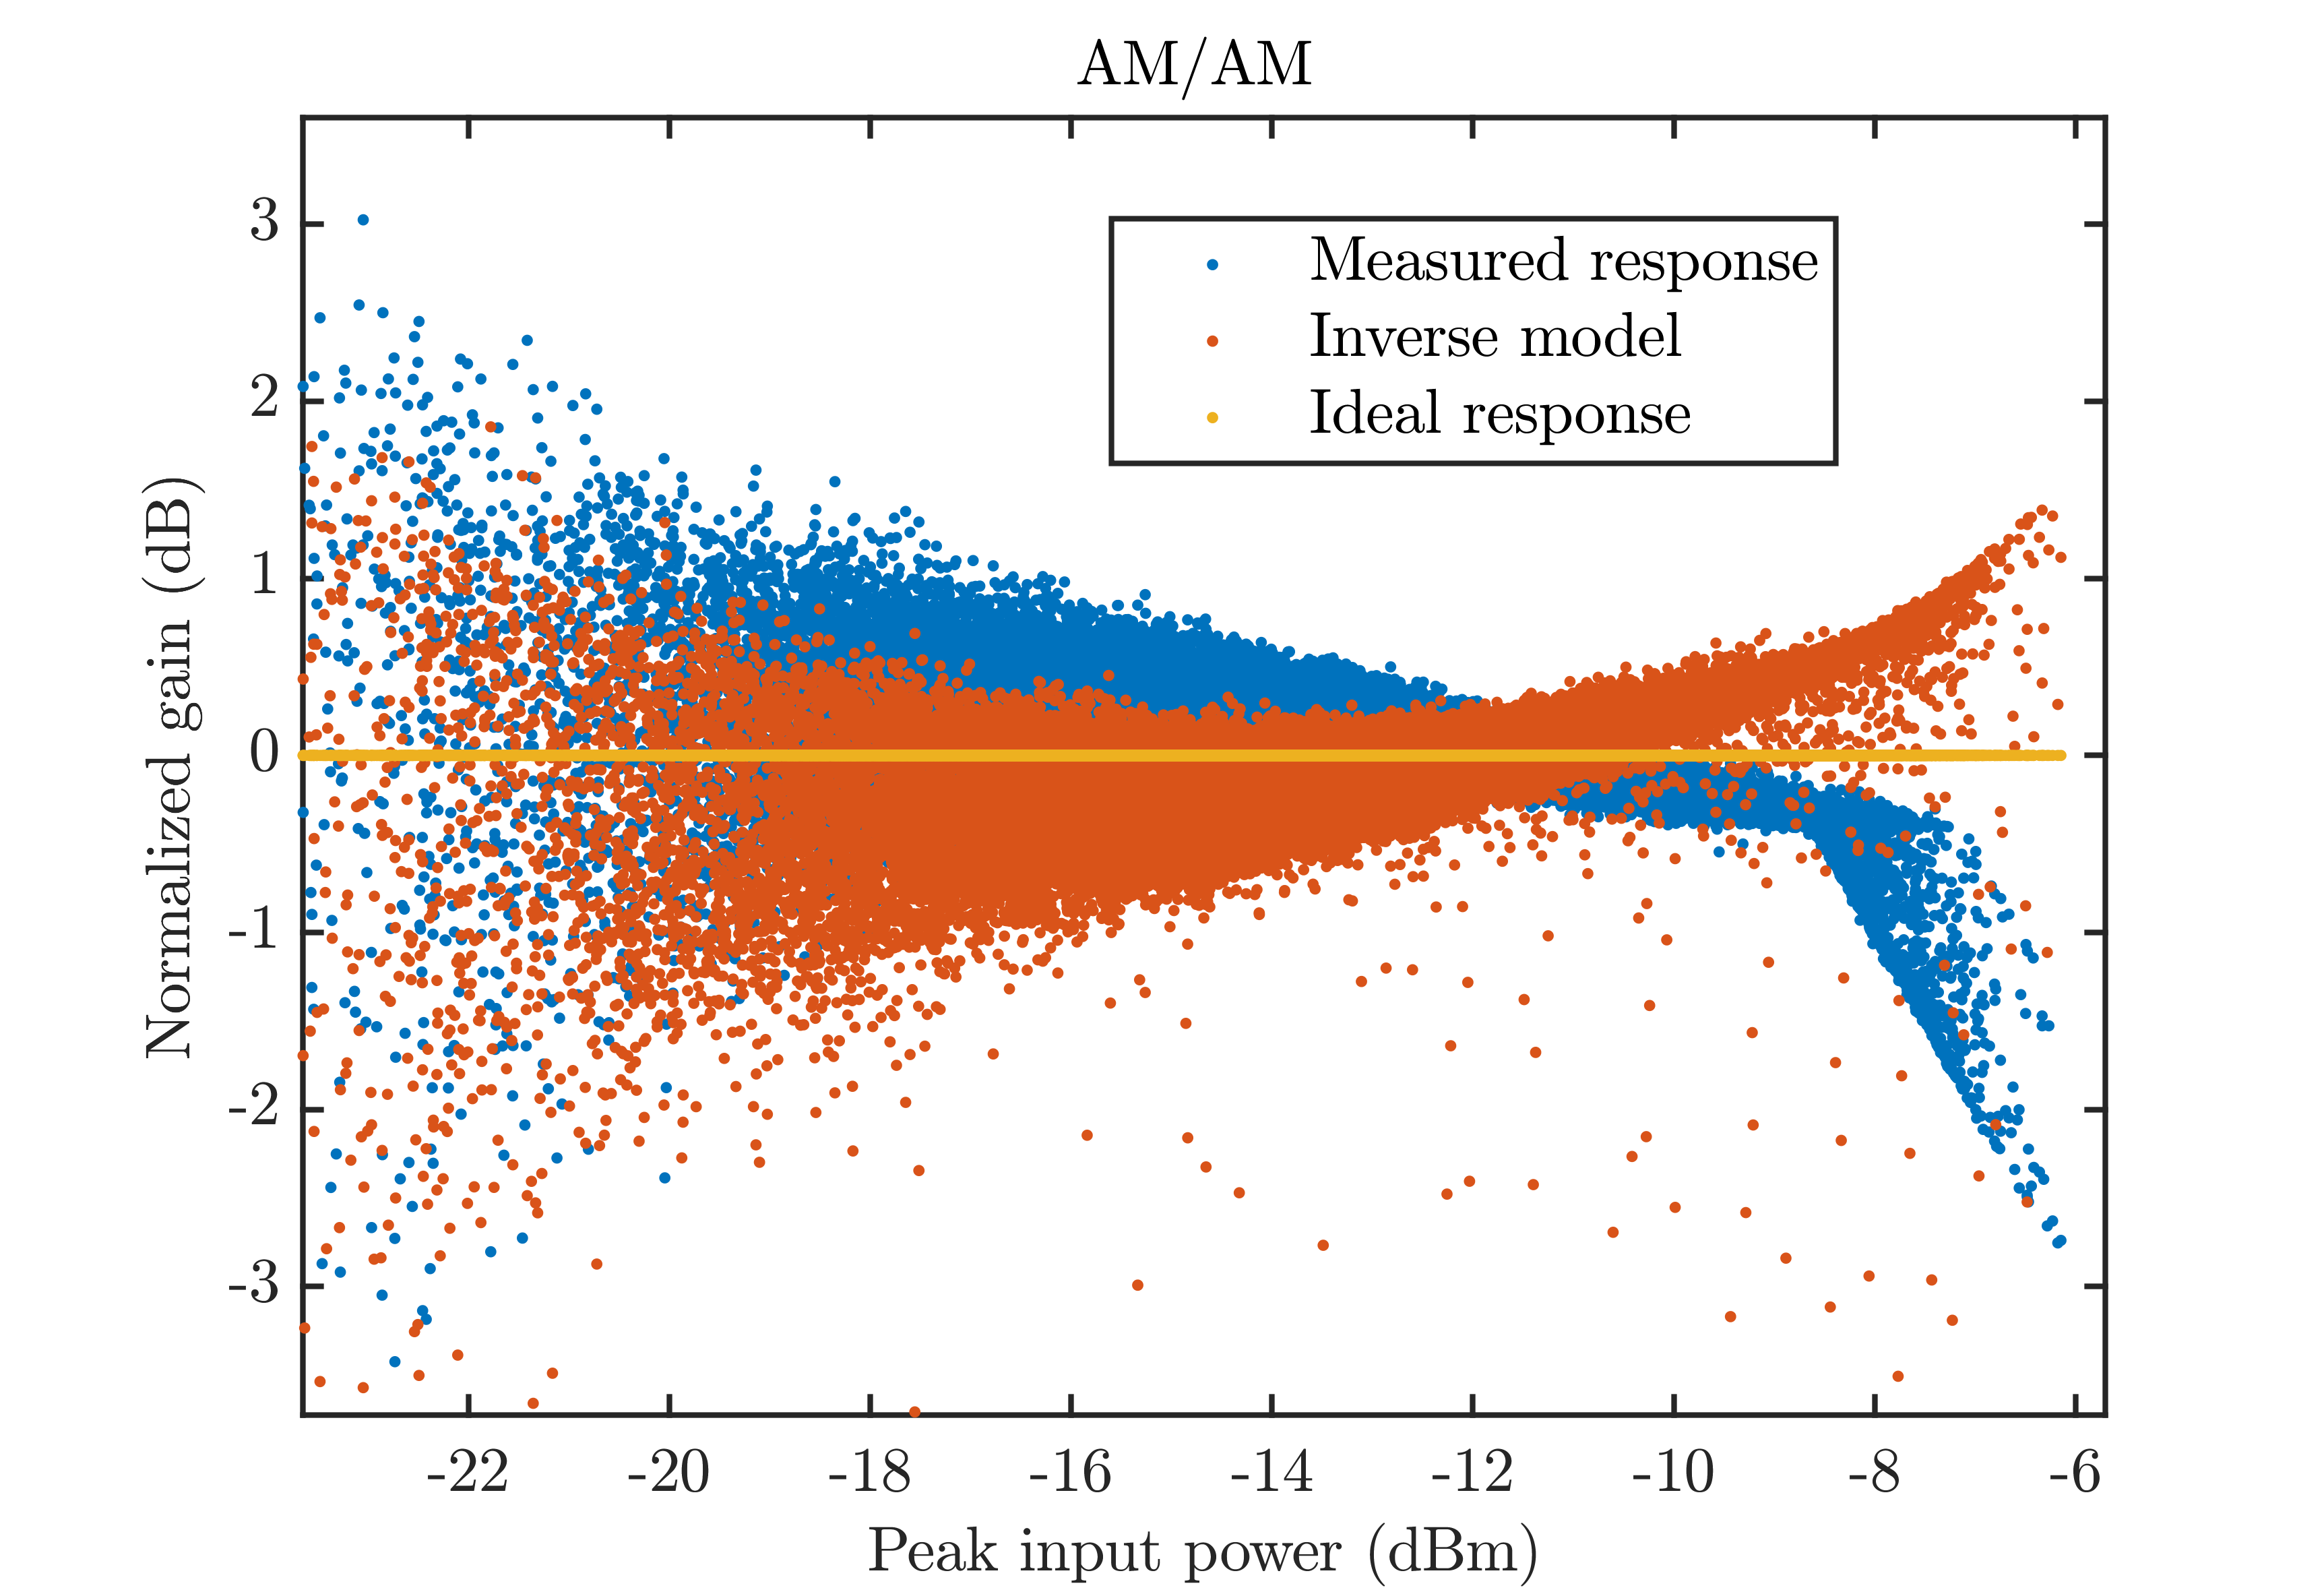
\includegraphics[scale = 0.7]{figures/measurement/predis.png}
\caption{AM/AM plot of measured response and inverse model}
\label{fig:pre_cons}
\end{figure}

\begin{figure}[H]
\centering 
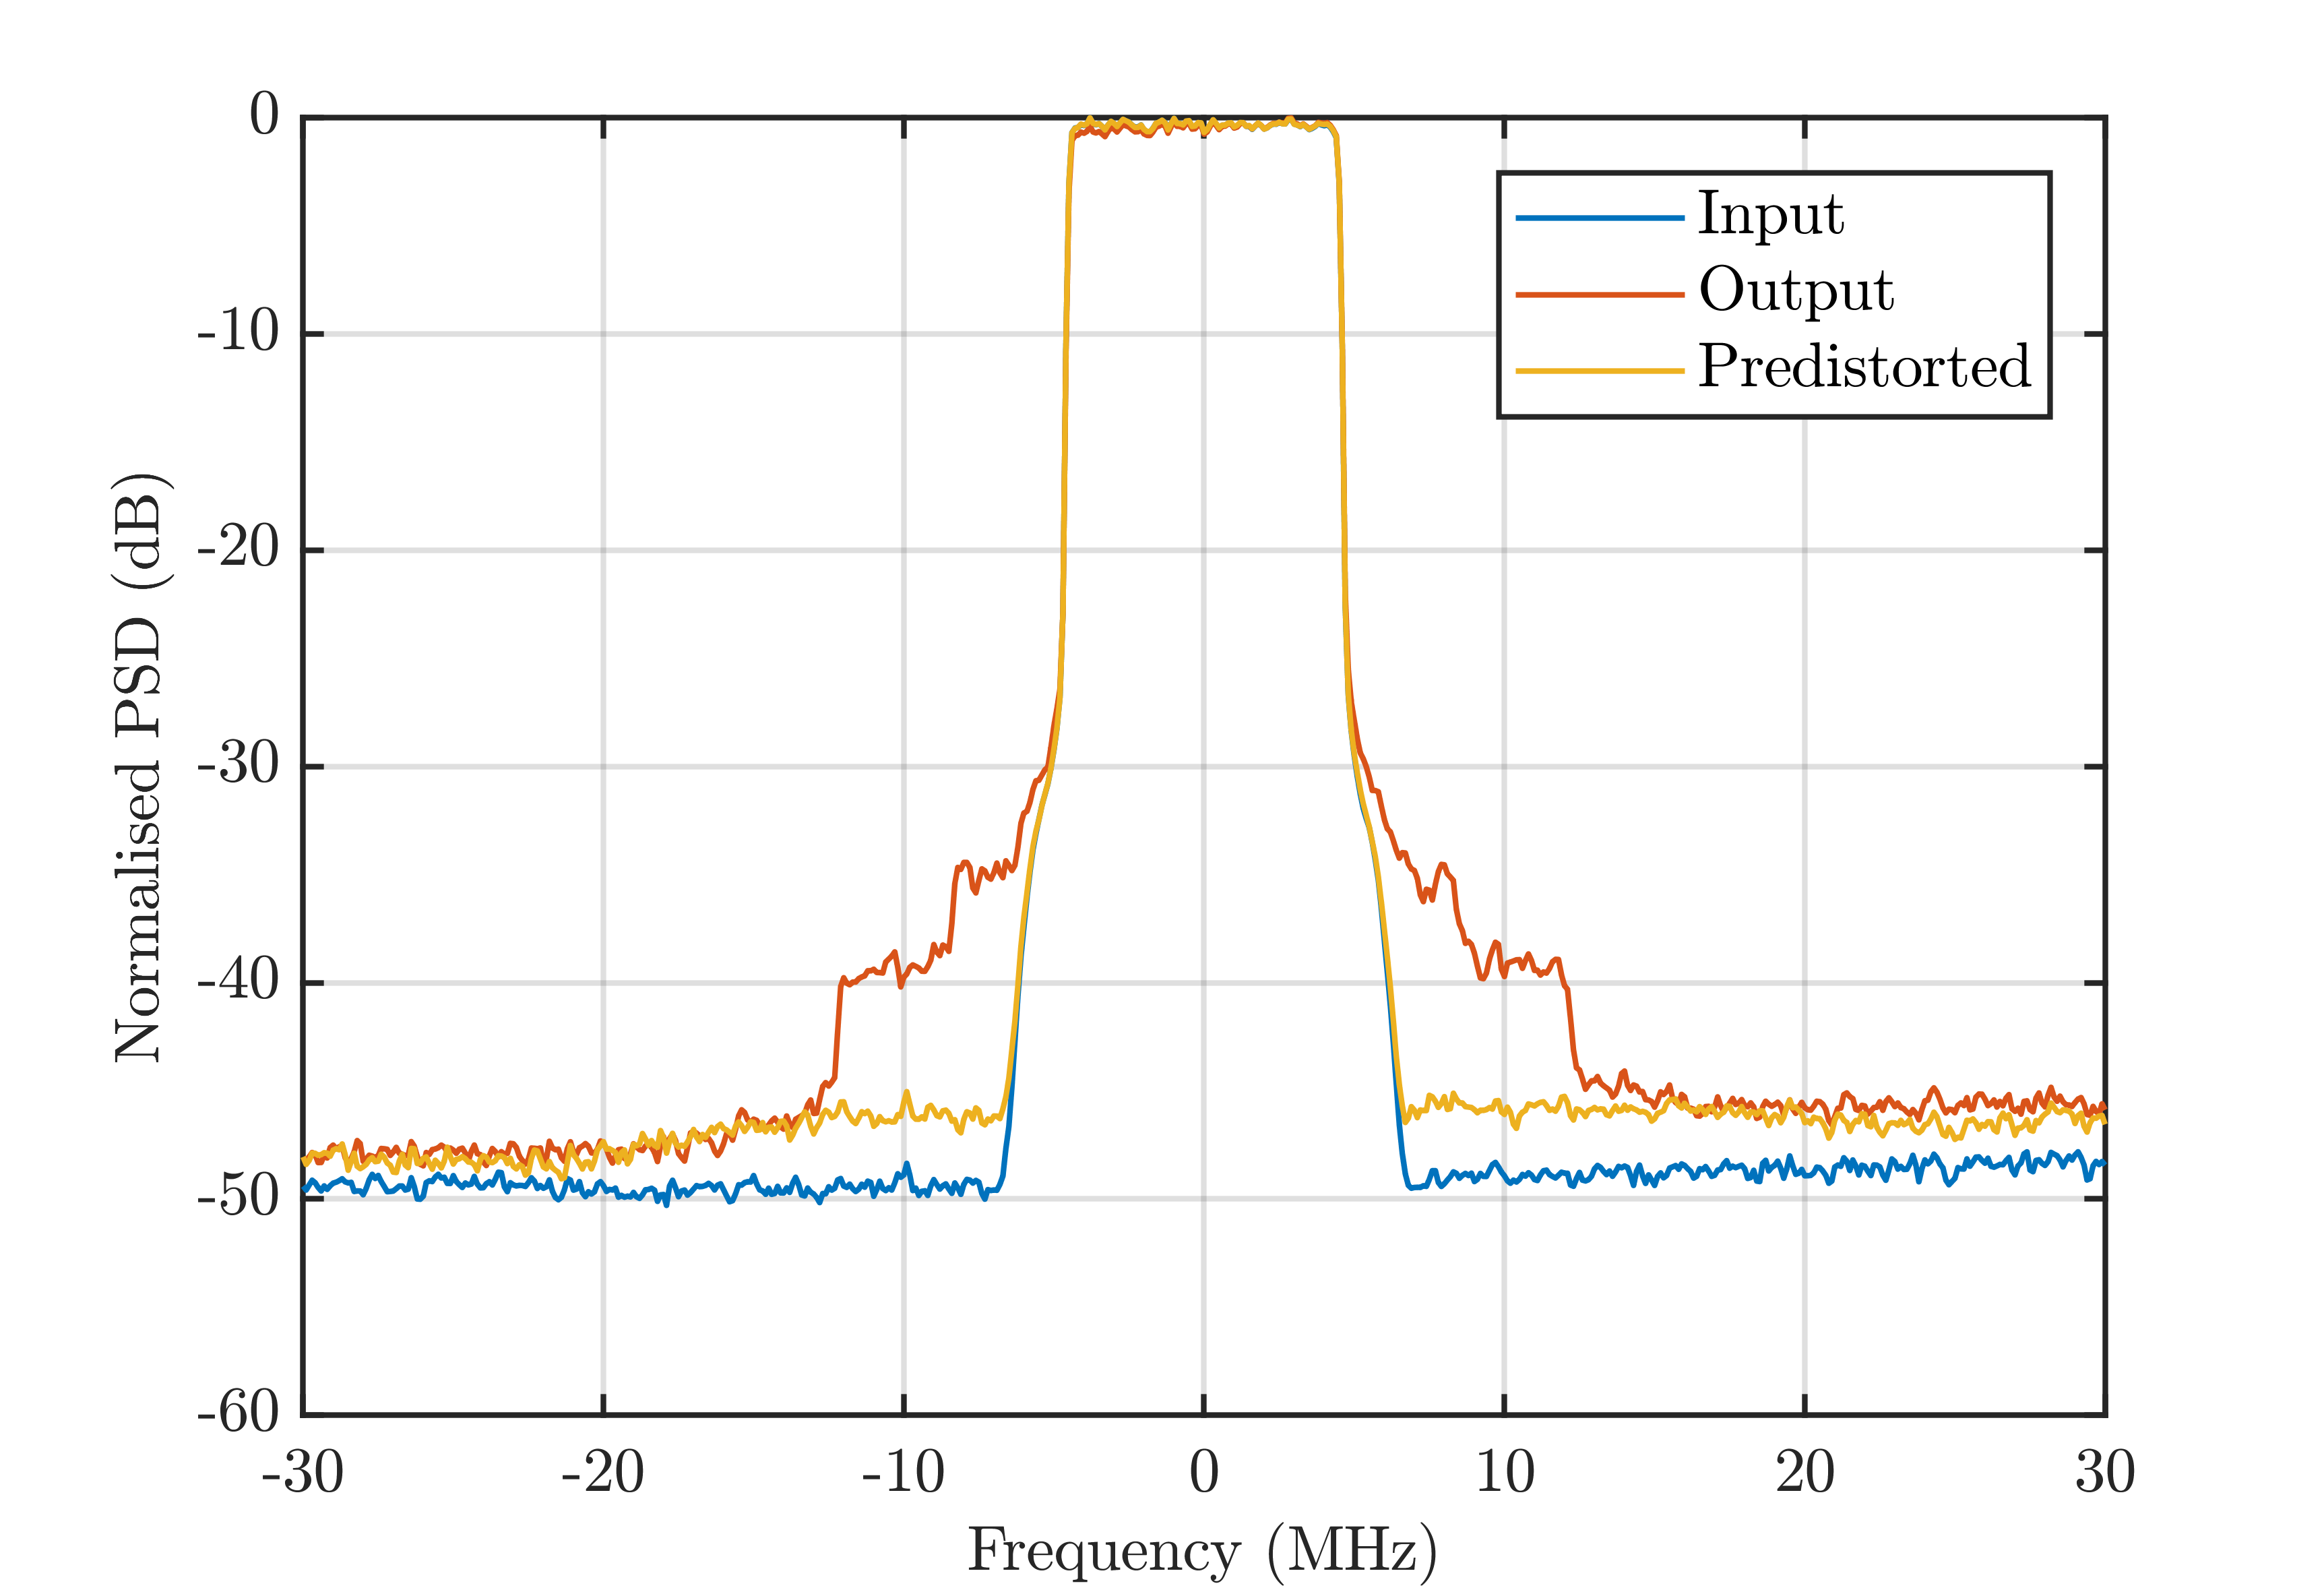
\includegraphics[scale = 0.7]{figures/measurement/psd_dpd.png}
\caption{PSD of output, input and inverse model}
\label{fig:pre_cons}
\end{figure}

\begin{figure}[H]
\centering 
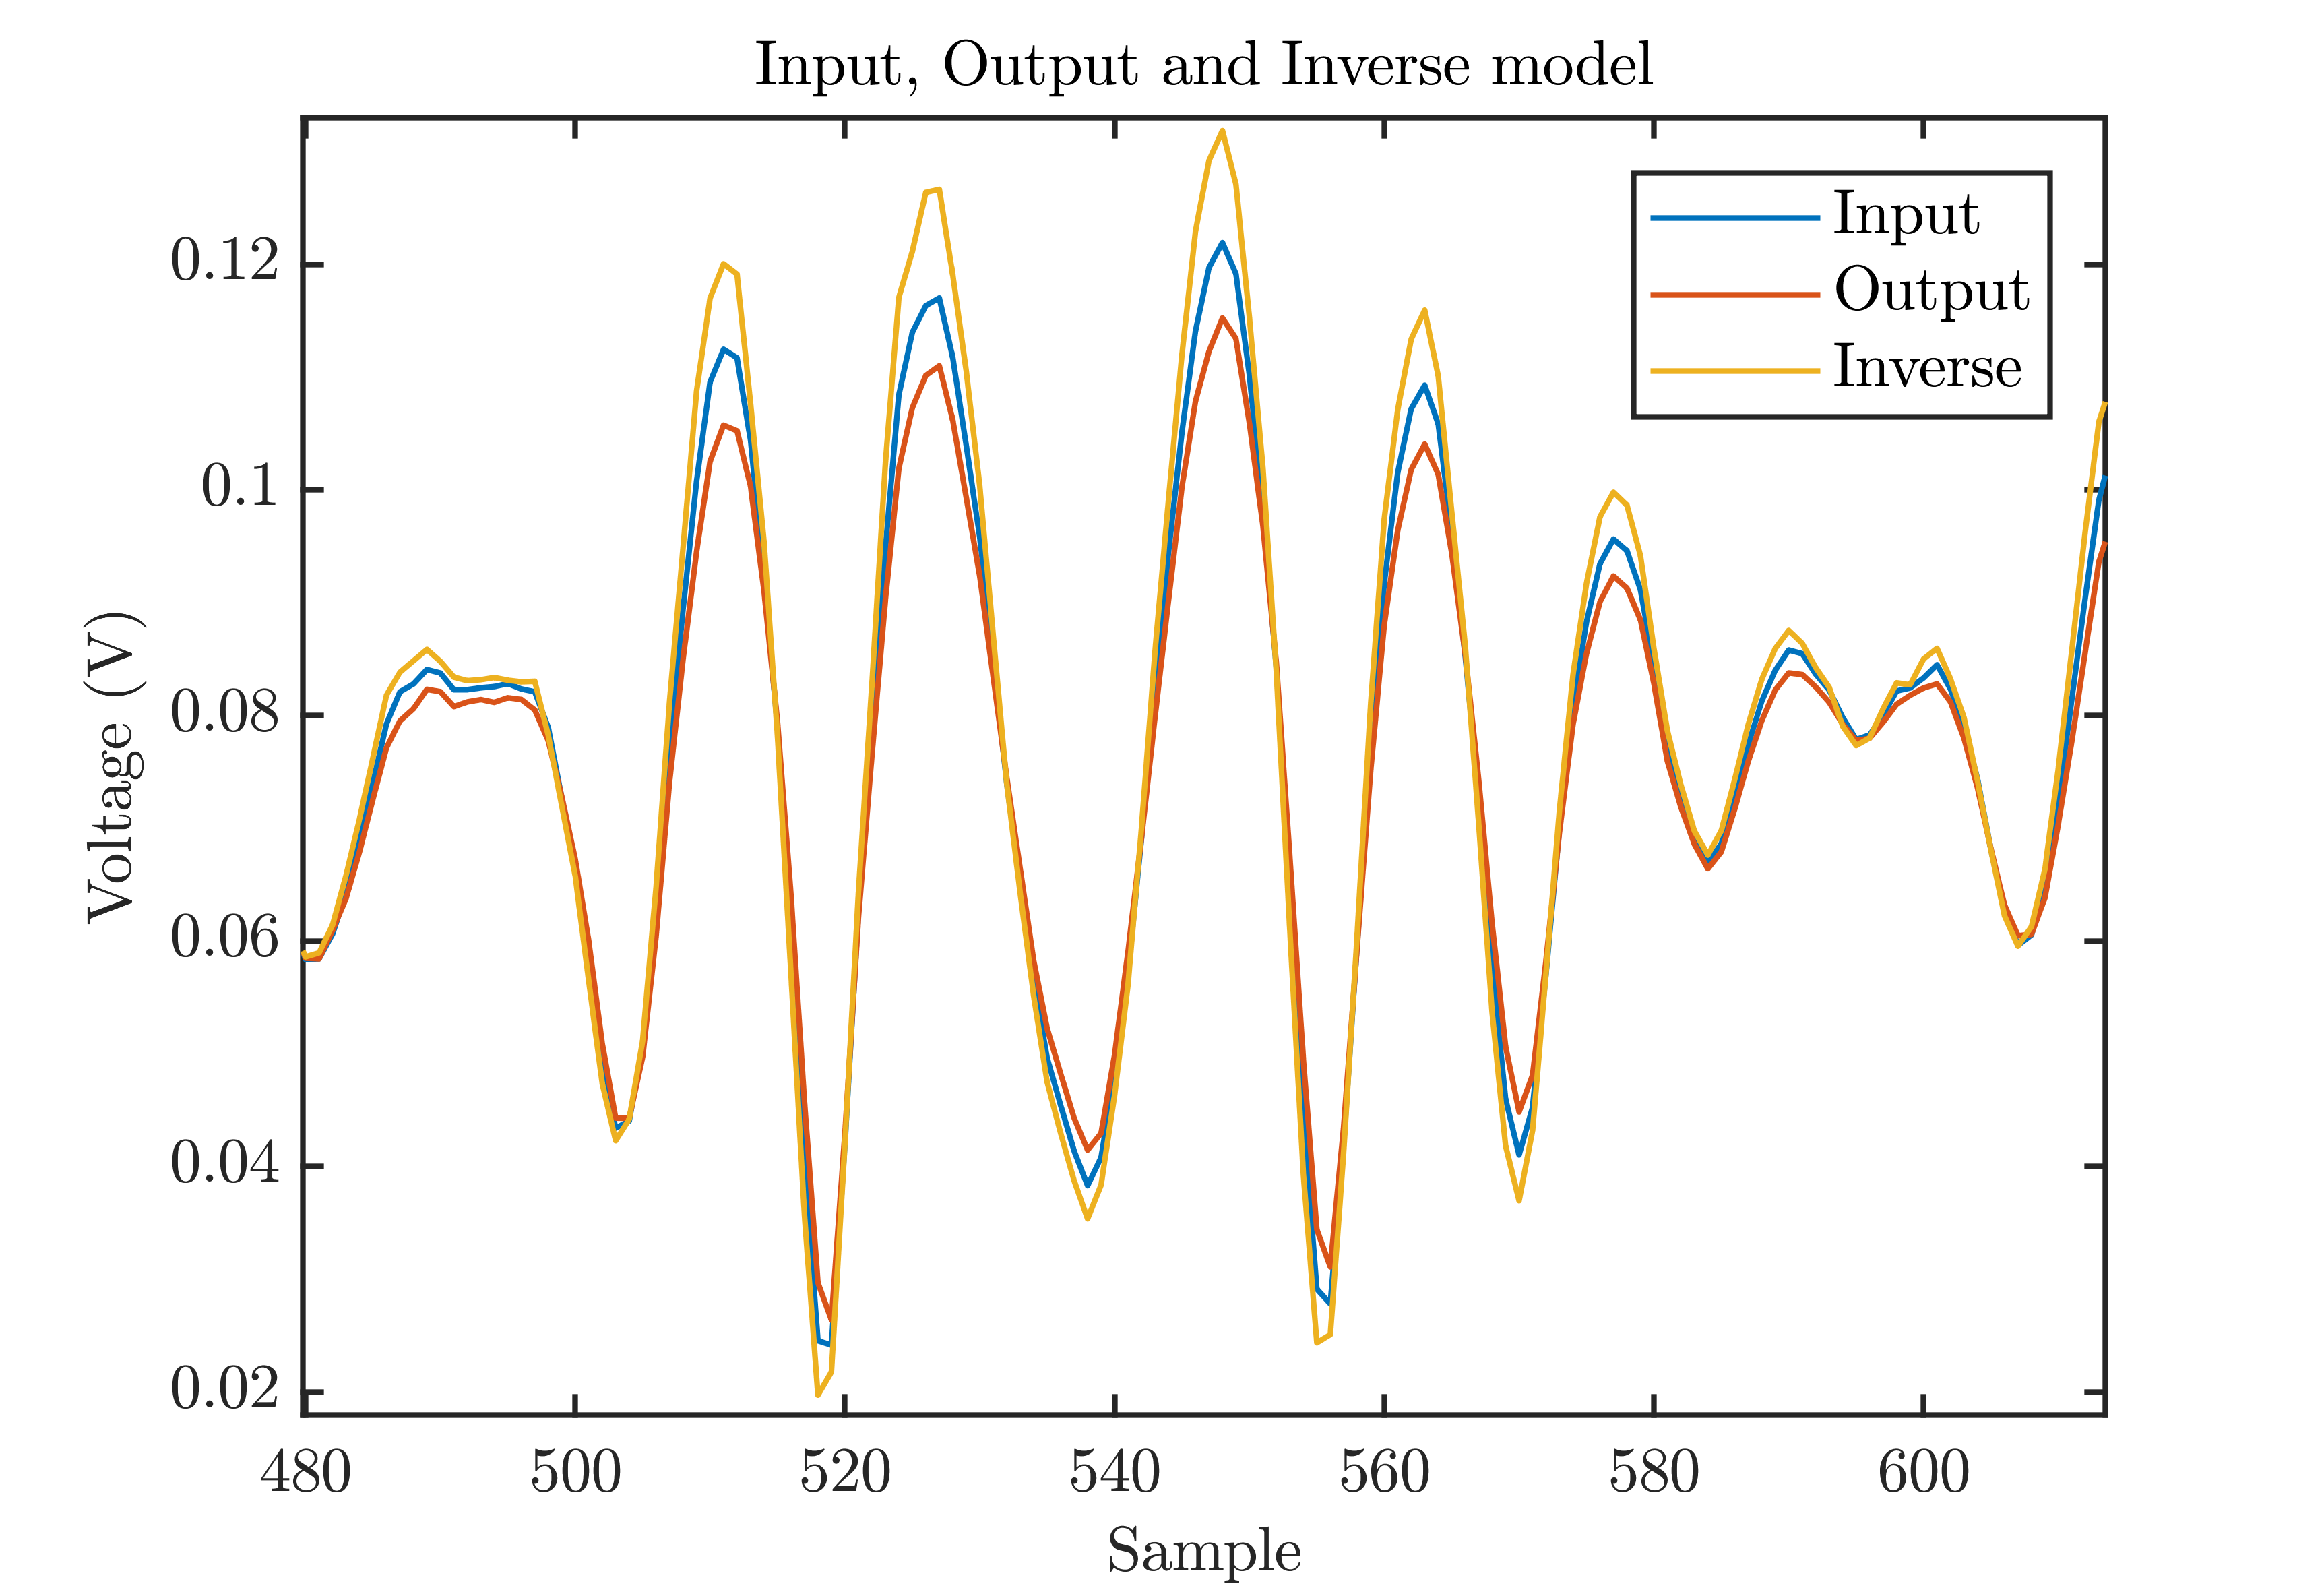
\includegraphics[scale = 0.7]{figures/measurement/inoutmodel.png}
\caption{Baseband signal of input, output and inverse model}
\label{fig:pre_cons}
\end{figure}

%%%%%%%%%%%%%%%%%%%%%%%%%%%%%%%%%%%%%%%%%%%%%%%%%%%%%%%%%%%%%%%%%%%%%%%%%%%%%%%%%%%%%%%%%%%%%%%%%%%%%%%%%%%%%%%%%%     


\section{Crosstalk}
Crosstalk is coupling from one branch to another branch. When only a signal is present on a single branch, no crosstalk would appear to this branch. On the other hand if a signal is presented at two branches then crosstalk would appear to both of them. There exist three types of crosstalk which is: Crosstalk before the PA's, see figure \ref{fig:cross_bf}, Crosstalk after the PA's, see figure \ref{fig:cross_af} and Crosstalk on the antennas and mishmash due to coupling. Crosstalk before the PA is also called nonlinear since it is amplified by the non linear PA. The nonlinear crosstalk and the PA nonlinear response should be jointly
compensated by a predistorter to get a reliable system performance \citep{islam2017} denoted $\mu_k (.)$. The output from the branches would become that of equation \ref{eq:nonlin}.

\begin{equation} \label{eq:nonlin}
Y_{1k} = fk(uk(X_{11},X_{12},X_{13},X_{1k}))
\end{equation}   

Where X is the input signal, Y is the output and $fk$ is the PA response. 

\begin{figure}[H]
  \centering
  \begin{minipage}[b]{0.5\textwidth}
	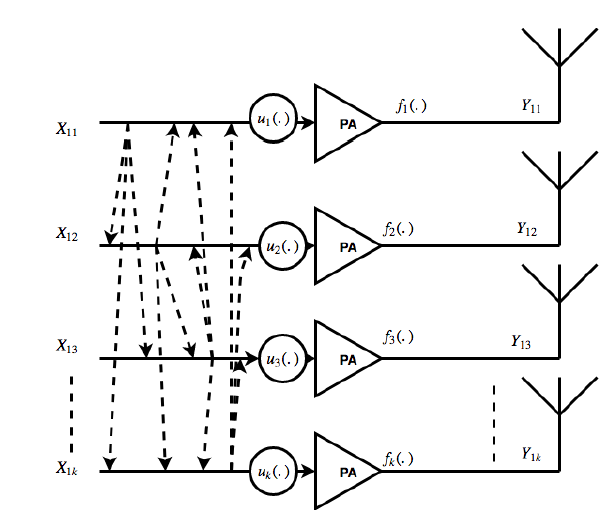
\includegraphics[scale = 0.5]{figures/ch1/crosstalk_before}
	\caption{Crosstalk before PA \citep{islam2017}}	
    \label{fig:cross_bf}
  \end{minipage}
  \hfill
  \begin{minipage}[b]{0.4\textwidth}
	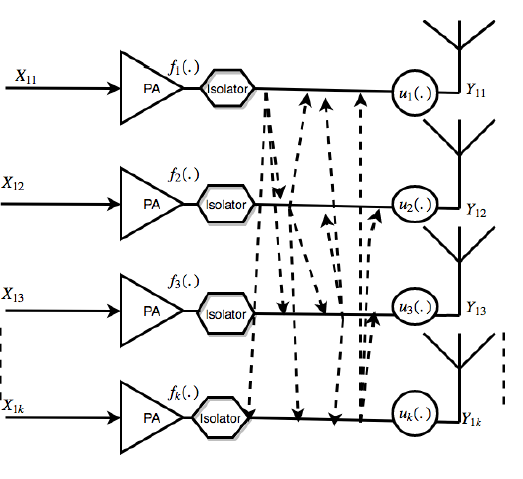
\includegraphics[scale = 0.5]{figures/ch1/crosstalk_after}
	\caption{Crosstalk after PA \citep{islam2017}}
    \label{fig:cross_af}
  \end{minipage}
\end{figure}

Crosstalk after the PA is called linear since it has an linear impact. In figure \ref{fig:cross_af} the output of the amplifier is connected to an isolator, which makes the output unaffected by reflections. A linear model can therefore be used which is shown in equation \ref{eq:lin_iso}. 

\begin{equation} \label{eq:lin_iso}
Y_{1k} = \mu_k(f1(X_{11}),f2(X_{12}),f3(X_{13})..fk(X_{1k}))
\end{equation}     

When no isolators is presented the output will now be affected by the crosstalk or mutual-coupling between the antennas. A sketch of this is depicted in figure \ref{fig:cross_ant} where $a_{1k}$ is the incoming signal to the amplifier, $b_{2k}$ is the output from the amplifier and $a_{2k}$ is the reflected signal form the antenna array at the k'th branch \citep{Hausmair2017}. The relation between $a_{2k}$
and the output signals $b_{2k}$ is determined by the characteristics
of the antenna array. The system model of the multi-antenna
transmitter can, therefore, be split in to a crosstalk and
mismatch model (CTMM). This block can further be used together with a dual-input-DPD which holds the model for the PA, see figure \ref{fig:cross_ctmm}. 


\begin{figure}[H]
  \centering
  \begin{minipage}[b]{0.5\textwidth}
	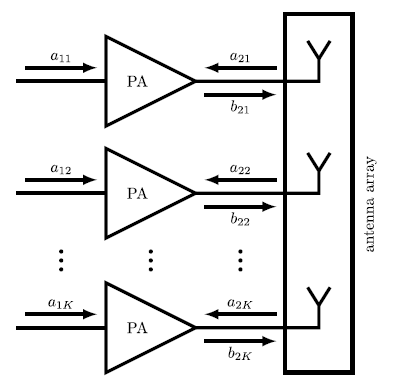
\includegraphics[scale = 0.5]{figures/ch1/crosstalk_antenna}
	\caption{Model of the antenna crosstalk \citep{Hausmair2017}}	
    \label{fig:cross_ant}
  \end{minipage}
  \hfill
  \begin{minipage}[b]{0.4\textwidth}
	\includegraphics[scale = 0.5]{figures/ch1/crosstalk_ctmm.png}
	\caption{The predistortion method consists of two main blocks: one linear CTMM block
for the whole transmitter and a dual-input DPD block in every transmit path. \citep{Hausmair2017}}
	\label{fig:cross_ctmm}
  \end{minipage}
\end{figure}




























